\documentclass[a4paper]{article}
\title{Praktikrapport - Universal Robots}
\author
{
    Johannes Ehlers Nyholm Thomsen\\ 
    \texttt{joha321j@edu.ucl.dk}
}

% Danish symbols.
\usepackage[utf8]{inputenc}
\usepackage[danish]{babel}
\usepackage[T1]{fontenc}

% Links and clickable ToC
\usepackage{hyperref}

% Images
\usepackage{graphicx}

\begin{document}

\maketitle

\newpage

\tableofcontents

\newpage

\section{Indledning}

\section{Forventninger}
Som led i datamatikeruddannelsen var jeg i et praktikforløb hos Bankdata.
I det praktikforløb blev jeg en del af et udviklingsteam,
hvor jeg hjalp dem med deres projekter.

Inden praktikforløbet hos Universal Robots(UR) startede, havde jeg en forventing om,
at det ville forløbe på samme måde.
Jeg så frem til at arbejde i et område,
der ikke var lige så konservativt som finansverdenen.
Jeg havde specifikt gået efter et firma,
der arbejdede i en anden sektor end Bankdata for at få et bredere syn på,
hvad jeg ville kunne arbejde med, når jeg var færdiguddannet.

\subsection{Læringsmål}
Jeg har haft opstillet nogle mål for, 
hvad jeg gerne ville have ud af mit praktikforløb hos UR.
Målene har hjulpet mig med at klargøre over for mig selv,
hvad jeg har af forventninger til mig selv under praktikforløbet.

I store træk gik læringsmålene ud på, 
at jeg gerne ville blive bedre til at være en del af et selvstyrende
udvilkingsteam.

\subsubsection*{Personlige Læringsmål}
\begin{itemize}
    \item Få mere erfaring i at indgå fagligt og professionelt i en 
    softwareudviklingsvirksomhed
    \item Forbedre mine evner i at deltage i et professionelt selvstyrende 
    udviklingsteam
    \item Få erfaring med brug af \href{https://en.wikipedia.org/wiki/OKR}{OKR's}
     til at opsætte og organisere mit teams mål for vores produkt.
\end{itemize}

\subsubsection*{Tekniske Læringsmål}
Mine tekniske læringsmål er opstillet på baggrund af en liste af teknologier
som teamet, jeg ville blive en del af, brugte.

\begin{itemize}
    \item Forbedre mine evner som full stack udvikler i .NET teknologi stacken
    \begin{itemize}
        \item Rest API udvikling med ASP.NET Core
        \item Single page application(SPA) udvilking med Blazor
        \item Brug af Entity Framework som Object Relational Mapper(ORM)
    \end{itemize}
    \item Forbedre mine evner inden for OpenAPI dokumentation ved brug af
    Swagger
    \item Få erfaring og kompetencer inden for brug af ElasticSearch
    \item Få erfaring inden for brug af MongoDB
\end{itemize}

Som alle ved overlever en god plan ikke længere end første møde med fjenden,
og jeg har derfor ikke opnået alle de læringsmål, som jeg har beskrevet her.
Se afsnit \ref{praktikforloeb} for en forklaring på hvorfor.
Dog har jeg lært en helt masse andet, 
som jeg vil komme ind på i afsnit \ref{udbytte}.

\section{Praktikforløbet}
\label{praktikforloeb}
I dette afsnit vil jeg beskrive selve praktikforløbet.
Først vil jeg beskrive, hvordan den daglige organisering var.
Dernæst vil jeg komme med eksempler på arbejdsopgaver.

\subsection{Ejet produktteam}
På første dag i praktikken blev jeg indformeret om,
at jeg ikke ville blive en del af myUR - Fleet.
myUR - Fleet er det produktteam, som jeg fik at vide under praktikinterviewet,
at jeg ville blive en udvikler hos.

I stedet fik Kasper, Mike og jeg at vide,
at vi 3 ville lave vores ejet produktteam.
Dernæst fik vi en problemstilling, som vi skulle løse.

\subsubsection{Problemstilling}
Universal Robots er inden for det sidste år skiftet struktur til at være 
produkt-orienterede i stedet for projektorienterede.
I den forbindelse har de forsøgt at give deres teams mere selvstyre ved at 
adoptere OKR's.

Kort fortalt går OKR's ud på, 
at den øverste ledelse sætter overordnede mål for virksomheden.
Ud fra de mål sætter afdelingerne mål for,
hvordan de kan hjælpe ledelsen med at opnå deres mål.
Til sidst sætter produktteamsne mål for, 
hvordan de kan hjælpe deres afdeling med at opnå afdelingens mål.
På denne måde har produktteamet selv ansvar for,
hvordan de giver værdi til virksomheden.

En del af OKR's er key results. 
Key results er målbare resultater, der skal bruges til at se,
om produktteamet er på vej mod deres mål.

Problemet var, at der var ingen god måde at visualisere 
fremskridtene for produtkteamsne.
Derfor var det svært for teamsne og se, hvordan det går med at opnå deres mål.

\subsubsection{Løsning}
I samarbejde med vores mentor, Julian, blev vi enige om, at vi skulle lave en 
løsning, der kunne tage i mod data og visualisere det i form af 
grafer, tabeller og lign.

\subsection{Organisering}
Julian og hans kollega Dennis ville være vores produkt owners,
mens vores chef Mark ville være vores stakeholder.
Ellers var Kasper, Mike og jeg fuldstændigt selvstyrende.

\subsubsection{Internt i teamet}
Vi fik et confluence rum, som vi har brugt til at dele forskellige filer, 
domæne modeller og wireframes blandt andet.

\begin{figure}[h!]
    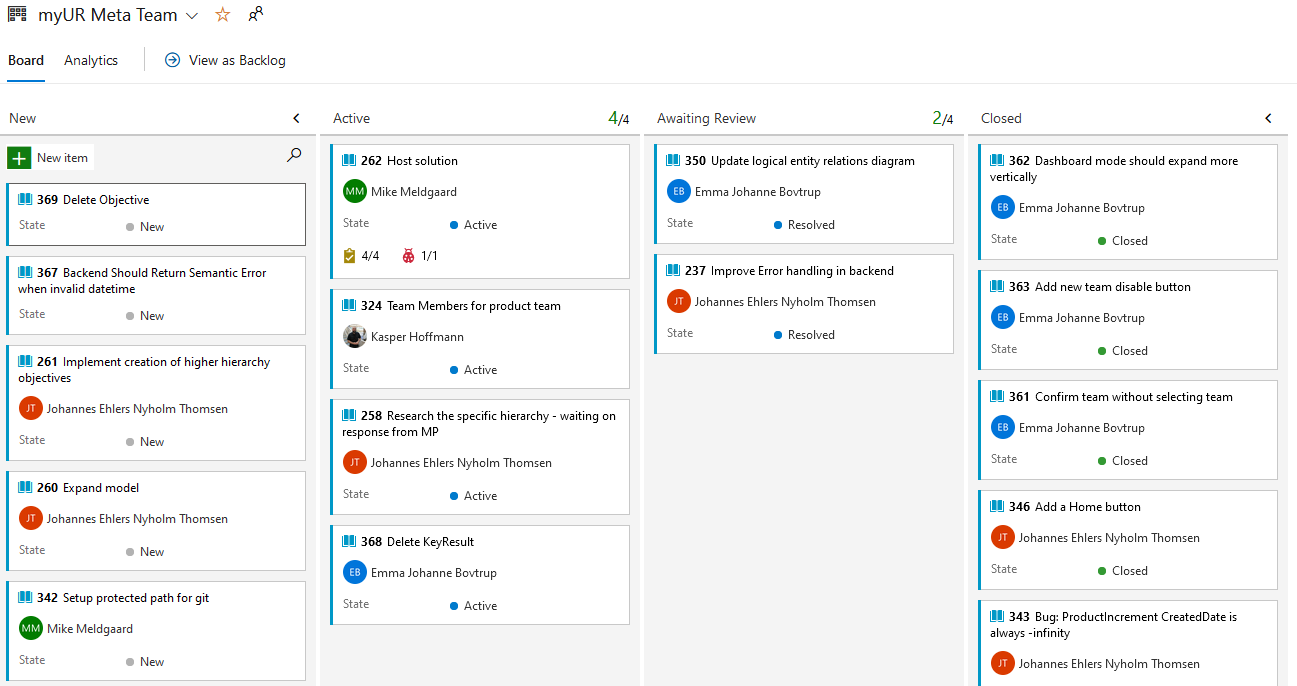
\includegraphics[width=\linewidth]{kanbanboard.png}
    \centering
    \label{kanban}
    \caption{Eksempel på vores kanban board}
\end{figure}

Til den daglige styring og organisering af vores arbejde
har vi brugt en Azure DevOps portal.
Vi brugte et Azure Board som et kanban-board
til at organisere det daglige arbejde, se figur \ref{kanban}.

Vi holdte daglige stand up møder.
Og hver anden uge holdte vi et retrospektiv for at sikre,
at vi blev ved med at blive bedre til at arbejde sammen.

Vi opstillede også kodestandarder, som vi lagde på confluence.
På den måde ville alle i teamet have adgang til dem,
og vi kunne også nemt løbende opdatere dem.
En del af vores standarder var,
at alt kode skal reviewes af et andet teammedlem.
For at sikre det opstillede vi regler,
så der ikke kunne pushes direkte til vores main branch.

\subsubsection{Resten af UR}
Jeg skal indrømme, at da jeg først hørte,
at vi ville blive vores ejet selvstændige hold,
var jeg bange for,
at vi ville blive parkeret i et hjørne og glemt indtil de 3 måneder var gået.
Heldigvis gjorde Mark, Julian og Dennis det hurtigt klart for mig,
at jeg tog fejl.

Julian og Dennis deltog i vores daglige stand ups.
Der var de begge rigtigt gode til at komme med deres syn på løsninger til blokerende opgaver.

Julian arrangerede også, at vi holdte en demo hver anden uge.
Under demoen kom de med feedback og idéer til forbedringer for vores produkt.
Mark deltog også i demoerne.

Vores afdeling af UR holdte også et all-hands møde en gang i kvartalet,
hvor hvert team præsenterede, hvad de arbejdede med.
Det skulle vi også,
og til mødet var der stor interesse for vores produkt.

\subsection{Full Stack udvilking}
Da vi var et selvstændigt udvilkingsteam betød det også,
at vi havde ansvaret for alt udvikling af vores produkt
lige fra frontend til database.

\subsubsection{Teknologi Valg}
Det første vi skulle gøre var at blive enige om,
hvilke teknologier vi ville bruge.
Til dette var Julian og Dennis en stor hjælp som sparingspartnere.
Det var nemmere at tage valgne,
når de kunne fortælle,
hvad der blev brugt i virksomheden.
Det handlede om at vælge det rigtige værktøj til opgaven,
men når vi stod med 2 lige gode værktøjer,
var det oplagt at bruge det samme værktøj som vores kollegaer.

\paragraph{Database}
Som database havde vi først tænkt på at bruge en MongoDB dokument database.
Det blev dog tydeligt for os, da vi satte os mere end i vores problemdomæne,
at vores data havde for mange relationer til, at det ville blive en success.

Derfor valgte vi at bruge en SQL database.
Tidligt i udvilkingsforløbet brugte vi blot en SQLite database.
Vi var dog nød til at gå væk fra en SQLite database,
da dens integration med Grafana ikke er særligt god.

I stedet valgte vi at bruge en PostgreSQL database.
Julian og Dennisses team var igang med at migrere fra en MongoDB til en PostgreSQL.
Derfor valgte vi at bruge det i stedet for et af alternativerne,
så det var nemt at udveksle erfaringer med dem.

\paragraph{Backend}
Det var oplagt at bruge .NET til vores backend,
da det blev brugt i resten af URs webløsninger.
Derfor ville vi have rig mulighed for at få hjælp
og udveksle erfaringer med de andre teams.

Som ekstra bonus var det et sprog, 
vi alle tre havde rig erfaring med at bruge grundet vores uddannelse.

\paragraph{Frontend}
Til frontenden valgte vi at bruge Blazor.
Vi valgte det,
da vi alle tre tidligere på uddannelsen havde arbejdet med Razor Pages,
og derfor havde vi erfaring med at bruge C\# til at skrive frontend.

Vi følte heller ikke, at det ville give et bedre produkt for UR,
hvis vi gav os igang med at lære at bruge Angular, React eller Vue.js.

\paragraph{Tye}
For at gøre det nemmere for os at udvikle en distribueret applikation
valgte vi at bruge et værktøj, der hedder
\href{https://github.com/dotnet/tye}{Tye}.
Tye gjorde det meget nemmere for os at udvikle,
da det selv kunne køre vores applikationer op med én kommando.
Alt hvad var nødvendigt var,
at vi havde lavet en yaml fil,
hvor vi fortalte Tye,
hvilke applikationer skulle køres op.
Et udsnit af vores yaml fil kan ses på figur \ref{tye}.

Tye understøttede også hotreloading både af vores frontend og backend,
da begge var .NET applikationer.

\paragraph{Grafana}


\section{Udbytte}
\label{udbytte}
\subsection{Selvstyring}
\subsection{Ny Teknologi}
\subsubsection{Integration med Grafana}

\end{document}